%%%%%%%%%%%%%%%%%%%%%%%%%%%%%%%%%%%%%%%%%
% University/School Laboratory Report
% LaTeX Template
% Version 3.1 (25/3/14)
%
% This template has been downloaded from:
% http://www.LaTeXTemplates.com
%
% Original author:
% Linux and Unix Users Group at Virginia Tech Wiki 
% (https://vtluug.org/wiki/Example_LaTeX_chem_lab_report)
%
% License:
% CC BY-NC-SA 3.0 (http://creativecommons.org/licenses/by-nc-sa/3.0/)
%
%%%%%%%%%%%%%%%%%%%%%%%%%%%%%%%%%%%%%%%%%

%----------------------------------------------------------------------------------------
%	PACKAGES AND DOCUMENT CONFIGURATIONS
%----------------------------------------------------------------------------------------

\documentclass{article}
\usepackage[margin=1in]{geometry}
%\usepackage[version=3]{mhchem} % Package for chemical equation typesetting
\usepackage{siunitx} % Provides the \SI{}{} and \si{} command for typesetting SI units
\usepackage{graphicx} % Required for the inclusion of images
%\usepackage{} % Required to change bibliography style to APA
\usepackage[backend=bibtex,maxnames=1]{biblatex}
%\usepackage{amsmath} % Required for some math elements 
\usepackage{hyperref}
\usepackage{acronym}
\usepackage{multirow}
\usepackage{amsmath,amssymb}

%\usepackage[utf8]{vietnam}

\setlength\parindent{25pt} % Removes all indentation from paragraphs

%\renewcommand{\labelenumi}{\alph{enumi}.} % Make numbering in the enumerate environment by letter rather than number (e.g. section 6)

%\usepackage{times} % Uncomment to use the Times New Roman font

%----------------------------------------------------------------------------------------
%	DOCUMENT INFORMATION
%----------------------------------------------------------------------------------------

\title{Conditional Table Generative Adversarial Network:\\ On solving the problem of high cardinality} % Title

\author{\textsc{Anh-Dung} Dinh} % Author name

\date{\today} % Date for the report

\bibliography{sample}
\begin{document}

\maketitle % Insert the title, author and date
\newacro{AI}{Artificial Intelligence}
\newacro{GANs}{Generative Adversarial Networks}
\newacro{CTGAN}{Conditional Table Generative Adversarial Networks}
\newacro{PacGAN}{Packing GAN}
\newacro{VGM}{Variational Gaussian Mixture model}
\begin{center}
\begin{tabular}{l r}
Supervisor: & Prof. Ngai-Man Cheung \\% Instructor/supervisor
& Dr. Ngoc-Trung Tran
\end{tabular}
\end{center}

% If you wish to include an abstract, uncomment the lines below
% \begin{abstract}
% Abstract text
% \end{abstract}
\tableofcontents
%----------------------------------------------------------------------------------------
%	SECTION 1
%----------------------------------------------------------------------------------------

\section{Introduction}

The problem of generating data has long attracted the great attentions from erudite scientists and scholars around the world. It could alternate traditional data, especially, when data is hard to achieve manually, and could provide adequate labels for training data as well instead of existing labelling data methods. This would result in extreme development in machine learning and \ac{AI} in the future due to its solution to the dearth of training data. In generative problems, one of very challenging and promising problems is to generate table data because of the seminal applications of synthetic table data. Usually, table data contains a lot of private information of users, businesses and governments. The publicity of this data, therefore, is impossible and dangerous which might confine researchers from doing experiments on this type of data. As a result, synthetic data is expected to keep the characteristics of the original data while keeping important information private so that the researchers could approach these data without concerning about privacy. 

In general, there are a number of methods could help to produce synthetic data that is expected to match the distribution of the original data. Some of them are Bayesian methods \cite{chow1968approximating} \cite{zhang2017privbayes}, others are \ac{GANs} \cite{choi2017generating} \cite{srivastava2017veegan} \cite{park2018data}. Although \ac{GANs} could perform well on images as it learn the implicit distribution effectively, the performance of \ac{GANs} on table data is unexpectedly poor. The reason for this is that the table data often keep the mixture of continuous features and discrete features which are different from other homogeneous types of data such as images or texts. In order to solve this problem, a method has been proposed in \cite{xu2019modeling} which is named as \ac{CTGAN}. This method provides a modelling way for both discrete and continuous data based on one-hot vectors. The performance shown in the paper \cite{xu2019modeling} is better than other \ac{GANs} \cite{choi2017generating} \cite{srivastava2017veegan} \cite{park2018data} and Bayesian methods \cite{chow1968approximating} \cite{zhang2017privbayes}. However, this input modelling method causes a very chronic problem which is high cardinality problem. If the number of features inside one column of the table data is too large, the one-hot vector becomes extremely long. As a result, the perennial mode collapse appears which facilitates the learning of "0" digits instead of the "1" digits due to the low frequencies of "1" digits. This causes poor performance for \ac{CTGAN} and need solving before this model could be applied in real-world problem as the real dataset often contains a lot of high cardinality features. In this work, we focus on solving the problem of high cardinality in table data generation. 

\section{Background}

In this section, we would go through several popular methods for generating tabular data including \ac{GANs} and Bayesian methods. 

 In \cite{choi2017generating}, the authors propose a method for generating patient records data. In this work, \citeauthor{choi2017generating} solve the problem of learning discrete data of \ac{GANs} by modelling the data into frequencies matrix. However, this method is too specific on medical data and patient records which could not perform on normal table data with mixture continuous and discrete features.  

The work \cite{park2018data} proposes the way to model table data into a square matrix by reshaping the vector into two dimensions matrix. After that, padding method is applied to make all matrices have the same size. the DCGAN is applied in this work to generate synthetic data as DCGAN was the stable and reliable model for generating data. 

On another approach, The VeeGAN in \cite{srivastava2017veegan} enhance the generative learning by a vector reconstructor network which is absolutely efficient in avoiding mode collapse. However, the VeeGAN suffers from the modelling the input for the table data as previous methods as other \ac{GANs}. As a result, the method could not results in good solution for generating table data which includes both discrete and continuous value.  The Figure \ref{fig:background} shows the results of these networks compared to Bayesian methods. 

\begin{figure}[h]
	\centering
	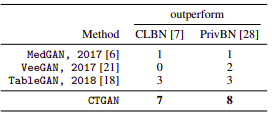
\includegraphics[scale=0.8]{figures/background.png}
	\caption{The number of wins of a particular methods compared with the corresponding Bayesian network against an appropriate metric on 8 real datasets. \cite{xu2019modeling}}
	\label{fig:background}
\end{figure}

\section{Conditional Table Generative Adversarial Networks}\label{ktcs}

The architecture of \ac{CTGAN} is similar to other \ac{GANs} models which includes a Generator $\mathbf{G}$ and a Discriminator $\mathbf{D}$. These two networks will try to compete with each other to achieve the better quality of the synthetic data. The Discriminator will try to distinguish the generated data with the original training data. On the other hands, the Generator will try to fool the Discriminator into accepting the generated data as the real data. 

\subsection{Generator and Discriminator}\label{subsec:gendis}

\subsubsection{Generator}
\begin{figure}[h]
	\centering
	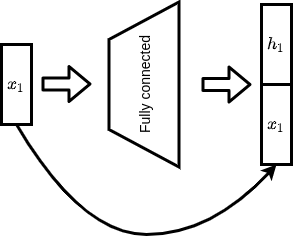
\includegraphics[scale=0.4]{figures/res.png}
	\caption{Residual block}
	\label{fig:res}
\end{figure}

Generator of \ac{CTGAN} is built from several Residual block (illustrated in Figure \ref{fig:res}). Generator takes input as two vectors. The first vector is the latent vector $z$ and the second vector is conditional vector $cond$. This $cond$ vector is specified based on the frequencies of the input which will be described in details in \ref{subsec:inout}. The output of the Generator is $\hat{x}$ which has the same shape with the training data $x$.The generator network is illustrated in Figure \ref{fig:gen}. 

\begin{figure}[h]
	\centering
	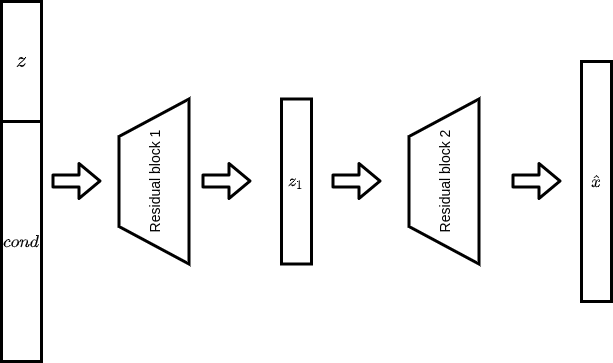
\includegraphics[scale=0.4]{figures/gen.png}
	\caption{Generator}
	\label{fig:gen}
\end{figure}

\subsubsection{Discriminator}

The Discriminator of \ac{CTGAN} is built from several fully connected layers. The input of the Discriminator is the concatenation of training data (could be real data $x$ or generated data $\hat{x}$) and the conditional vector. Output is a scalar value indicates the how close is the generated data to the original data. In order to avoid the mode collapse, \ac{PacGAN} is utilized to boost the performance, in which, more than one input vectors are concatenated to map to one scalar output value. The model of Discriminator is illustrated in Figure \ref{fig:dis}.

\begin{figure}[h]
	\centering
	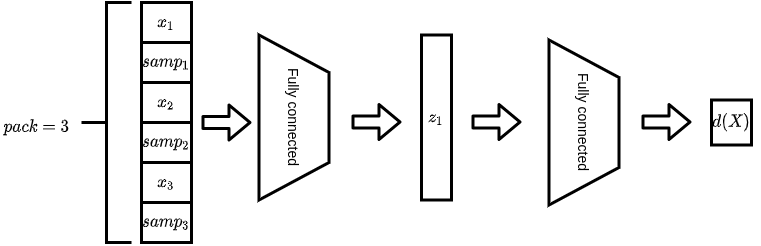
\includegraphics[scale=0.4]{figures/dis.png}
	\caption{Discriminator}
	\label{fig:dis}
\end{figure}


\subsection{Input and output}\label{subsec:inout}

One of the good advantages of \ac{CTGAN} is a modelling method for both discrete and continuous values. In this subsection, the method is described in details

\subsubsection{Continuous and discrete value}

\begin{figure}[h]
	\centering
	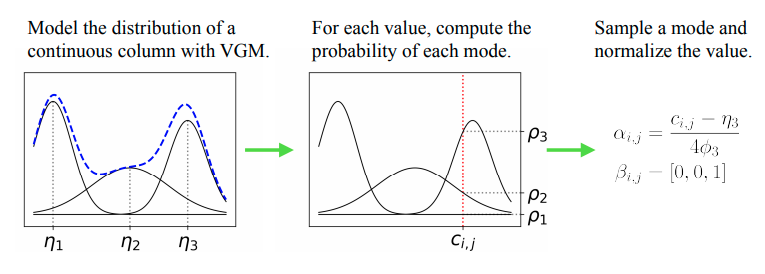
\includegraphics[scale=0.5]{figures/conmix.png}
	\caption{An example of mode-specific normalization}
	\label{fig:conmix}
\end{figure}

\begin{itemize}
	\item For each continuous column $C_i$, use \ac{VGM} \cite{bishop2006pattern} to estimate number of modes $m_i$ and fit a Gaussian mixture. For instance, in Figure \ref{fig:conmix}, the \ac{VGM} finds three modes ($m_i = 3$), namely $\eta_1, \eta_2, \eta_3$. The learned Gaussian mixture is $\mathit{P}(c_{i, j}) = \sum_{k=1}^{3}\mu_k\mathit{N}(c_{i,j}; \eta_k, \phi_k)$ .
	\item For each value $c_{i,j} \in C_i$, compute the probability of $c_{i,j}$ coming from each mode. For instance, in Figure\ref{fig:conmix}, the probability densities are $\rho_1, \rho_2, \rho_3$. The probability densities are computed as $\rho_k = \mu_k\mathit{N}(c_{i,j}; \eta_k, \phi_k)$.
	\item Sample one mode from give the probability density, and use the sampled mode to normalize the value. For example, in Figure \ref{fig:conmix}, we pick the third mode given $\rho_1, \rho_2, \rho3$. Then we present $c_{i,j}$ as a one hot vector $\beta_{i,j} = [0, 0, 1]$ indicating the third mode, and a scalar $\alpha_{i,j}= \frac{c_{i,j} - \eta_3}{4 \phi_3}$ to represent the value within the mode. 
\end{itemize}

From the method of representation above we have a row (\ref{equ:con}):

\begin{equation}\label{equ:con}
	r_j = \alpha_{1,j} \oplus \beta_{1,j} \oplus ... \oplus\alpha_{N_c, j} \oplus \beta_{N_c,j} \oplus d_{1, j} ... \oplus d_{N_d, j}
\end{equation}
Where:
\begin{itemize}
	\item $d_{i,j}$ is the one hot representation for the $i^{th}$ discrete value of the row $j$.
	\item ${N_c}$ is the number of continuous columns.
	\item ${N_d}$ is the number of discrete columns.
\end{itemize}

\subsubsection{Conditional vector}

In the subsection \ref{subsec:gendis}, we have introduced the conditional vector $cond$ which is concatenated with $x$ or $z$ to become the input of Discriminator or Generator. In fact, we have two types of conditional vectors, one is for Discriminator and the other is for the Generator. The conditional vector of Generator is denoted as $cond$ and the conditional vector of the Discriminator is denoted as $samp$.

\begin{figure}[h]
	\centering
	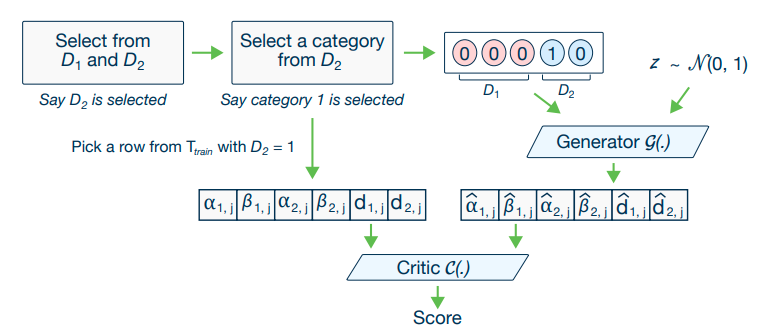
\includegraphics[scale=0.3]{figures/cond.png}
	\caption{An example of conditional vector}
	\label{fig:cond}
\end{figure}

$cond$ is constructed to indicate the condition $D_i^* = k^*$. Recall that all the discrete columns $D_1, D_2,..., D_{N_d}$ end up as one-hot vectors $d_1, d_2, ..., d_{N_d}$ such that the $i^{th}$ one-hot vector $d_i = [d_i^{(k)}], \forall k={1,..., |D_i|}$. Keep the same shapes of vectors $d_i$, we could construct list of one-hot vectors $m_1, m_2,..., m_{N_d}$ as:

\begin{equation}
	m_i^{(k)} = \begin{cases}
	1, \quad \text{if $i = i^*$ and $k=k^*$}\\
	0, \quad \text{otherwise.}
	\end{cases}
\end{equation}
The $k^*$ index is selected by several steps:
\begin{enumerate}
	\item Select the column $D_i$ out of all $N_d$ discrete columns, with equal probability. Let $i^*$ be the index of the column selected. For instance,in Figure \ref{fig:cond}, the selected column was $D_2$, so $i^* = 2$.
	\item Construct a PMF across the range of values of the column selected in the previous step, $D_{i^*}$, such that the probability mass of each value is the logarithm of its frequency in that column.
	\item Let $k^*$ be a randomly selected value according to the PMF above. For instance, in Figure 2, the range $D_2$ has two values and the first one was selected, so $k^*=1$.
\end{enumerate}

These vectors $m_i$ are called masked vectors. The $cond$ vector is built up by concatenating those mask vectors.

\begin{equation}
	cond = m_1 \oplus m_2 \oplus ... \oplus m_{N_d}
\end{equation}


Them $samp$ vector is constructed based on the $cond$ vector. $samp$ is picked from the real dataset with given $cond$ vector. For example, in Figure \ref{fig:cond}, we sample $samp$ vector with $D_2 = 1$. The purpose of $samp$ vector is to match the conditional distribution $\mathit{P_G}(row|cond)$ with $\mathit{P_D}(row|cond)$ through a generator loss defined in the next subsection.


\subsection{Losses}

\ac{CTGAN} includes three basic losses which are \ac{GANs} loss, generator loss and gradient penalty.
 \begin{itemize}
 	\item \textbf{GANs loss:} The loss of \ac{CTGAN} also based on the principle of minimax game as \ac{GANs}:
 	\begin{equation}
 	L_D = - \mathop{\mathbb{E}}[\log(\mathbf{D(x)})]  - \mathop{\mathbb{E}}[\log(1 - \mathbf{D}(\mathbf{G}(z \oplus cond)))]
 	\end{equation}
 	
 	\begin{equation}
 	L_G = - \mathop{\mathbb{E}}[\log(\mathbf{D}(\mathbf{G}(z \oplus cond)))]
 	\end{equation}
 	\item \textbf{generator loss:} The generator loss is to do two jobs. First, it adds penalty if the generated data $\hat{x}$ do not produce the value specified by the $cond$ vector. Second, it match the conditional distribution $\mathit{P_G}(row|cond)$ with $\mathit{P_D}(row|cond)$. The function is based on the cross entropy loss:
 	\begin{equation}
 	L_{cond} = -samp * \log(\hat{x}) - ( 1- samp) * \log(1-\hat{x})
 	\end{equation}
 	
 	\item \textbf{gradient penalty:} 
 \end{itemize} 

\section{Improvements}

In this work, we try to solve the problem of learning high cardinality. The problem is caused by long one-hot vectors in the input which affects the learning performance.

\subsection{Quantization}

Quantization is a method to embed a one-hot vector into two dimensional matrix, and this matrix could be represented by two one-hot vectors. These two one-hot vectors will have much shorter length compared to the original vector. Hence, the problem of the high cardinality is partly solved. The results see an significant improvement. 

The Table \ref{tab:quant} shows the experimental results of quantization. The quantization give the best performance when it is applied on high cardinality column. In case that we do quantization on low cardinality column, the results see a slightly fall compared to non-quantization encoding method. The results also emphasize the high score if the data do not contain high cardinality columns. 

\begin{table}[htpb]\centering
	\begin{tabular}{|c|c|c|c|c|}
		\hline
		\multirow{2}{*}{\textbf{Note}}           & \multicolumn{2}{c|}{\textbf{Score 1}} & \multicolumn{2}{c|}{\textbf{Score 2}} \\ \cline{2-5} 
		& \textbf{mean}      & \textbf{std}     & \textbf{mean}      & \textbf{std}     \\ \hline
		Quantize high card columns               & 677247.81          & 10242.60         & 836580.82          & 14898.64         \\ \hline
		No quantization               & 655366.58          & 4803.44          & 766639.72          & 10350.19         \\ \hline
		Quantize low card columns + no high card & 694054.61          & 10252.27         & 864160.41          & 10439.23         \\ \hline
		no quantization + no high card           & 720837.77         & 7450.51          & 890978.35          & 9566.95          \\ \hline
	\end{tabular}
\caption{Experimental results on quantization on dataset Fire Department}
\label{tab:quant}
\end{table}


Although the improvement of the quantization method is significant, we could realize that quantization faces the problem of un-correlation learning problem. The Table \ref{tab:marbox} shows the marginal distribution difference between synthetic dataset and original dataset indicating low discrepancy. On the other hands, the Table \ref{tab:corbox} shows the conditional distribution difference between synthetic dataset and original dataset indicating high value. This might be caught by the un-correlation learning between quantized columns. 

\begin{table}[htpb] \centering
	\begin{tabular}{|c|c |c |}
		\hline
		\textbf{Note} & \textbf{Box 1} & \textbf{Box 2} \\ \hline
		Norm1         & 0.5628         & 0.7269         \\ \hline
		Norm2         & 0.0780         & 0.3071         \\ \hline
		AVG           & 0.0029         & 0.072          \\ \hline
		Max Norm 1    & 0.043,0        & 0.2527         \\ \hline
		KL            & 0.2268         & 0.338          \\ \hline
	\end{tabular}
\caption{Marginal distribution difference of each quantized columns between synthetic dataset and original dataset}
\label{tab:marbox}
\end{table}

\begin{table}[htpb]\centering
	\begin{tabular}{|c|c|c|}
		\hline
		\textbf{Note} & \textbf{Box1 | Box2}        & \textbf{Box 2 | Box 1}       \\ \hline
		Norm1         &  47.5325 &  57.9454 \\ \hline
		Norm2         &  5.6105  &  10.0445 \\ \hline
		AVG           &  0.0896  &  0.0712  \\ \hline
		Max Norm 1    &  1.9767  &  8.7491  \\ \hline
		KL            &  242.649 &  49.215  \\ \hline
	\end{tabular}
\caption{Conditional distribution difference of two quantized columns between synthetic dataset and original dataset}
\label{tab:corbox}
\end{table}


\subsection{Binning}

Binning is a method for compressing the long one-hot vector into a shorter one. The value between each collapsed step is uniformly selected in decoding phase. 


\begin{table}[htpb]\centering
	\begin{tabular}{ccccccc}
		\hline
		& \multicolumn{3}{c}{\textbf{Binning}}                         & \multicolumn{3}{c}{\textbf{Quantization}}                    \\ \hline
		\textbf{Binning}           & \textbf{Score 1}   & \textbf{Score 2}   & \textbf{Average}   & \textbf{Score 1}   & \textbf{Score 2}   & \textbf{Average}   \\ \hline
		No Binning or quantization & 655366.58          & 766639.72          & \textbf{711003.15} & 655366.58          & 766639.72          & 711003.15          \\ \hline
		50                         & 630987.22          & 821657.07          & 726322.15          & \textbf{655846.89} & \textbf{830462.44} & \textbf{743154.67} \\ \hline
		100                        & 642242.63          & 818245.73          & 730244.18          & 653309.45          & 824114.80          & 738712.12          \\ \hline
		150                        & 635489.74          & 818261.19          & 726875.47          & 644840.36          & 826304.16          & 735572.26          \\ \hline
		200                        & 635074.67          & 817888.62          & 726481.64          & 638408.05          & 823820.32          & 731114.18          \\ \hline
		300                        & \textbf{640771.98} & \textbf{825294.32} & \textbf{733033.15} & 646626.32          & 827551.52          & 737088.92          \\ \hline
		400                        & 634798.32          & 825758.36          & 730278.34          & 642151.26          & 824041.117         & 733096.19          \\ \hline
		500                        & 632569.55          & 817560.17          & 725064.86          & 646402.11          & 823043.16          & 734722.63          \\ \hline
	\end{tabular}
\caption{Comparison between binning and quantization (bold value indicates best performance of the selected method)}
\label{tab:binbox}
\end{table}

The Table \ref{tab:binbox} shows the experimental results of the application of binning and quantization method on different ranges. In comparison, the quantization performs slightly better than the binning method. 

Since the improvement of the quantization over binning method is not so significant, we could predict that the second quantized column of the quantization method has learned trivial features. This is because the binning and quantization method shares the same first column, the binning method would randomly choose value in the leap to get the original value, while the quantization keep the second column. This problem is illustrated in Figure \ref{fig:conadd}. The conditional distribution learned given first column value is not matched with the original distribution.


\begin{figure}[h]
	\centering
	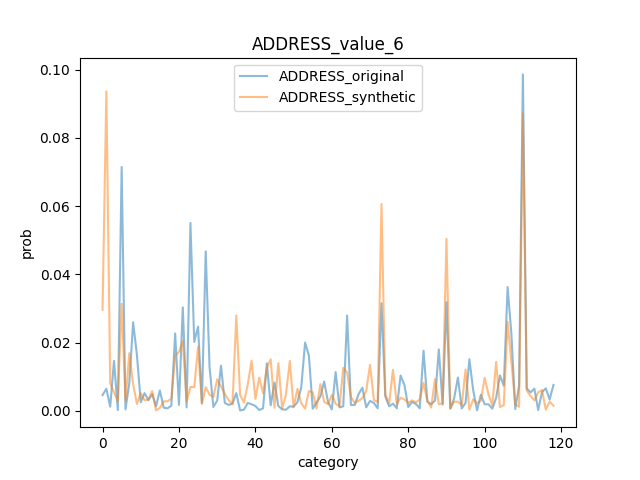
\includegraphics[scale=0.6]{figures/conadd.png}
	\caption{Conditional distribution of second column value given the first column value (with 16000 records)}
	\label{fig:conadd}
\end{figure}

\subsection{Gumbel training}

One of the characteristics of \ac{CTGAN} is to utilize the Gumbel Softmax \cite{jang2016categorical} which outputs an one-hot vector from a continuous vector. As a result, the two discrete quantized columns have to go through two Gumbel Softmax separately causing loss information. The idea of this work is to train Gumbel Softmax to output two-hot vectors instead of two one-hot vectors as before. (The results of this method are not good, so I will update this later)


\subsection{Normalization}

In this subsection, we discuss about the idea to normalize the high cardinality column into one continuous value. Here we define a threshold is the minimum number of features that the column is required to get normalization. For example with threshold is $5$, we will only normalize the columns with the number of features less or equal $5$. There are several ways we could normalize the results:

\begin{itemize}
	\item Norm from 0 to 1
		\begin{equation}
		norm_1(d_i) = \frac{d_i}{\max D}
		\end{equation}
	\item Norm from -1 to 1
		\begin{equation}
		norm_2(d_i) = \frac{d_i \times 2}{\max D} -1
		\end{equation}
		
\end{itemize}

 
 The experimental results show several interesting points. 

\subsubsection{Adult dataset}

On adult dataset, most of the columns are integer values. As a result, we could treat their distribution as a continuous distribution. We do so by normalizing the range of integer into the continuous range of $[0; 1]$. The experimental result is illustrated in the Table \ref{tab:normadult}. The results indicate slightly better performance of the normalization method compared to quantization.

\begin{table}[htpb]\centering
	\begin{tabular}{cccc}
		\hline
		\textbf{Threshold}      & \textbf{Score 1}   & \textbf{Score 2}   & \textbf{Average}   \\ \hline
		Binning or quantization & 656869.69          & 944483.75          & 800676.72          \\ \hline
		5                       & 491032.05          & 876792.20          & 683912.12          \\ \hline
		10                      & 502637.23          & 878922.35          & 690779.79          \\ \hline
		250                     & \textbf{669648.14} & \textbf{945911.72} & \textbf{807779.93} \\ \hline
	\end{tabular}
\caption{Comparison between different threshold of normalization on Adult dataset (bold value indicates best performance of the selected method)}
\label{tab:normadult}
\end{table}

\subsubsection{Fire Department}

On fire department dataset, we face an imbroglio that the discrete values are categorical not integer. As a results, the orders of categories in one-hot vectors affects the performance. In \ref{tab:normfire}, it could be seen that the performance of normalization be worse than quantization method results. The reason behind is the smooth distribution caused by the assumption of a continuous distribution over the column (illustrated in Figure \ref{fig:normbox}). 


\begin{figure}[h]
	\centering
	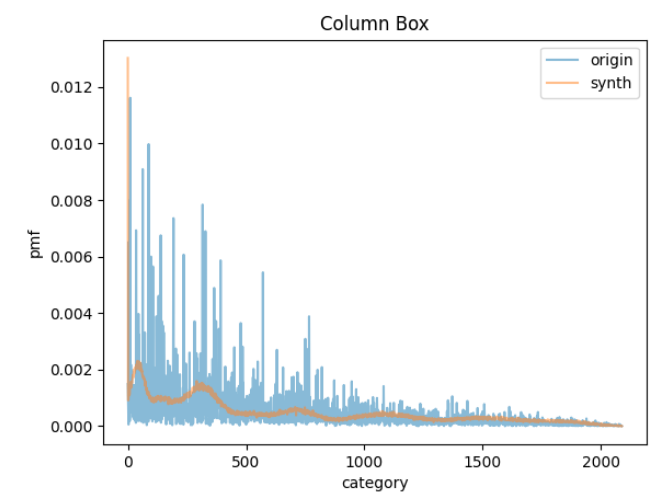
\includegraphics[scale=0.5]{figures/normbox.png}
	\caption{Plot a high cardinality column under the normalization method}
	\label{fig:normbox}
\end{figure}



\begin{table}[]\centering
\begin{tabular}{ccccc}
	\hline
	\textbf{Threshold} & \textbf{Score 1}   & \textbf{Score 2}   & \textbf{Average}   & \textbf{Number of normalized columns} \\ \hline
	None               & \textbf{655846.89} & \textbf{830462.44} & \textbf{743154.67} &                                       \\ \hline
	5                  & 598569.04          & 798215.59          & 698392.31          & 17                                    \\ \hline
	10                 & 585764.57          & 798385.45          & 692075.01          & 13                                    \\ \hline
	250                & 625458.35          & 818531.67          & 721995.01          & 2                                     \\ \hline
\end{tabular}
\caption{Comparison between different threshold of normalization on Fire Department dataset (bold value indicates best performance of the selected method)}
\label{tab:normfire}
\end{table}

\subsubsection{Sorting values before normalization}

In order to void the smooth distribution line, we sort the categories based on frequencies before normalizing into the continuous range. The result is quite positive. The Table \ref{tab:sortfire} shows a little improvement when we use the method of normalization with frequencies sorting. Furthermore, the figure \ref{fig:sortfire} also points out the extirpation of the smooth distribution of the synthetic data.

\begin{table}[htpb]\centering
\begin{tabular}{ccccc}
	\hline
	\textbf{Binning} & \textbf{Score 1}   & \textbf{Score 2}   & \textbf{Average}   & \textbf{Number of normalized columns} \\ \hline
	None             & \textbf{655846.89} & \textbf{830462.44} & \textbf{743154.67} & \multicolumn{1}{l}{}                  \\ \hline
	5                & 602986.33          & 764499.69          & 683743.01          & 17                                    \\ \hline
	10               & 602590.46          & 780597.81          & 691594.14          & 13                                    \\ \hline
	250              & \textbf{667385.56} & \textbf{825795.27} & \textbf{746590.41} & 2                                     \\ \hline
\end{tabular}
\caption{Comparison between different threshold of normalization with sorting frequencies on Fire Department dataset (bold value indicates best performance of the selected method)}
\label{tab:sortfire}
\end{table}


\begin{figure}[h]
	\centering
	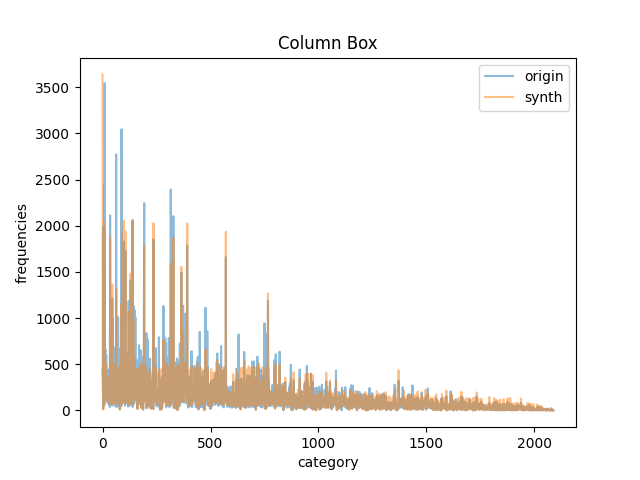
\includegraphics[scale=0.5]{figures/sortbox.png}
	\caption{Plot a high cardinality column under the normalization method}
	\label{fig:sortfire}
\end{figure}

\subsection{Latent Optimization}

While the small update in latent vector could cause some effects in generating image, we also take the concern to the same problem in generating table data. As a result, in this work, we try to update the latent vector to achieve better result.

From the Table \ref{fig:lo}, we could see that the change is not so significant, although we increase the learning rate for updating latent vectors. The updated vectors are illustrated in Figures \ref{fig:lo001}, \ref{fig:lo2e4} and \ref{fig:lo100}.


\begin{table}[htpb] \centering
	\begin{tabular}{cccc}
		\hline
		\multicolumn{1}{l}{} & \textbf{Score 1}   & \textbf{Score 2}   & \textbf{Average}   \\ \hline
		No LoGAN             & \textbf{649939.63} & 818272.22          & 734105.92          \\ \hline
		LoGAN + lr=2e-4      & 645794.84          & \textbf{827557.90} & \textbf{736676.37} \\ \hline
		LoGan + lr=0.01      & 646836.08          & 825865.88          & 736350.98          \\ \hline
		LoGan + lr=1         & 639779.08          & 826679.95          & 733229.52          \\ \hline
	\end{tabular}
\caption{Results on running CTGAN with latent optimization}
\label{fig:lo}
\end{table}


\begin{figure}[h]
	\centering
	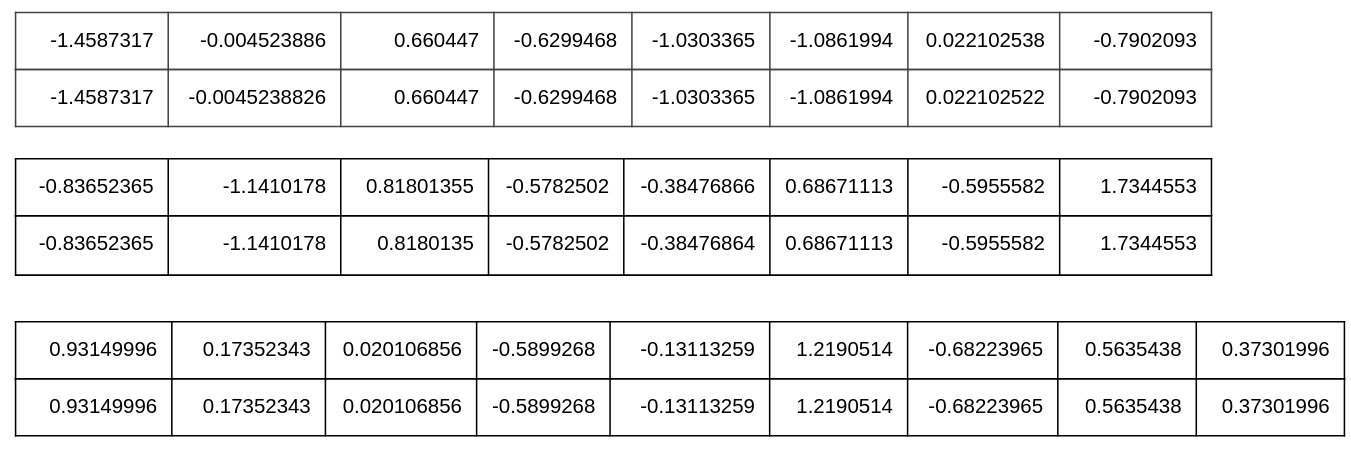
\includegraphics[scale=0.3]{figures/lo2e4.png}
	\caption{Latent vector update with learning rate = 2e-4 (lower vector is updated vector)}
	\label{fig:lo2e4}
\end{figure}

\begin{figure}[h]
	\centering
	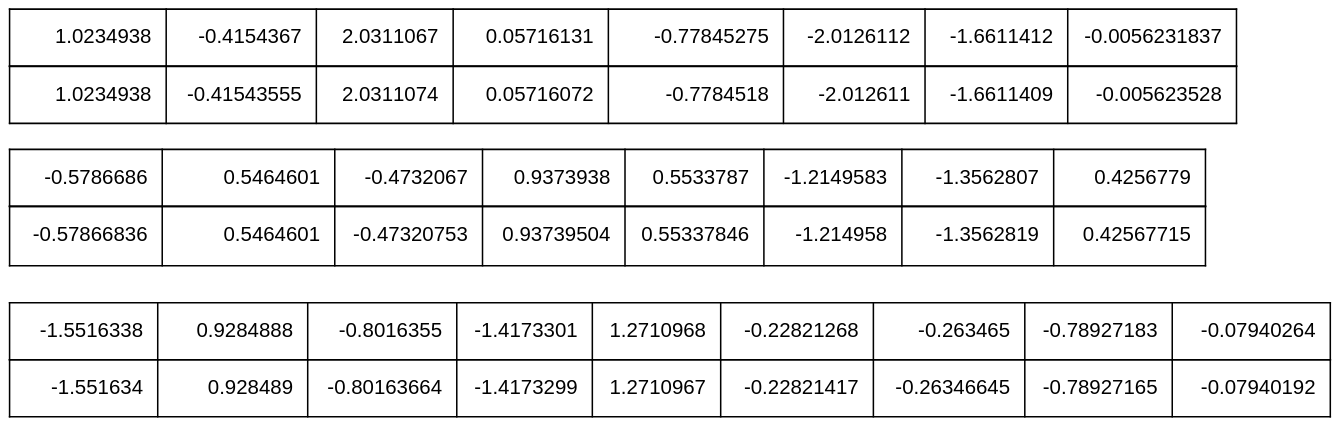
\includegraphics[scale=0.3]{figures/lo001.png}
	\caption{Latent vector update with learning rate = 0.01 (lower vector is updated vector)}
	\label{fig:lo001}
\end{figure}

\begin{figure}[h]
	\centering
	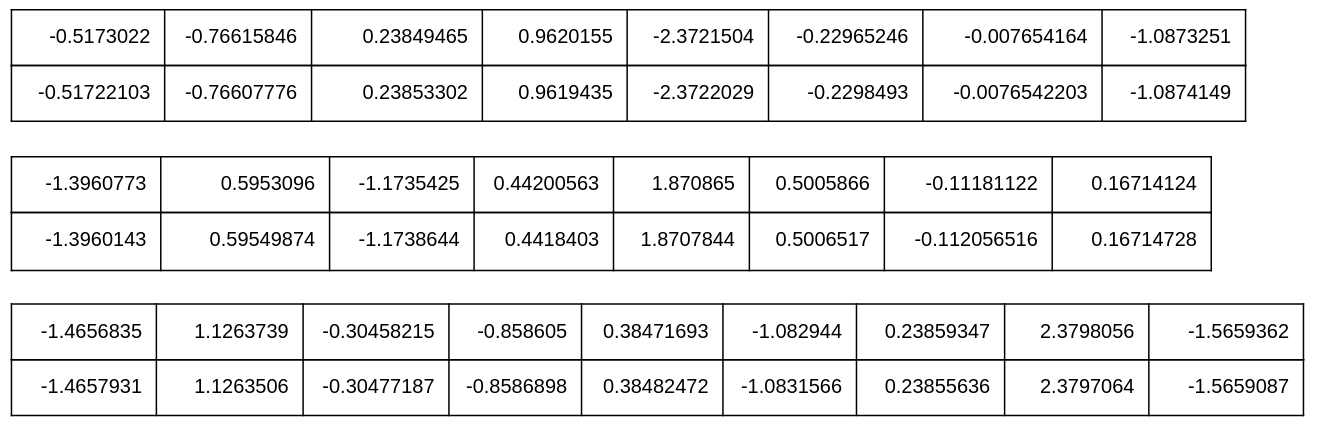
\includegraphics[scale=0.3]{figures/lo100.png}
	\caption{Latent vector update with learning rate = 100 (lower vector is updated vector)}
	\label{fig:lo100}
\end{figure}

\printbibliography

%----------------------------------------------------------------------------------------


\end{document}